\documentclass[11pt,a4paper,notitlepage]{article}
\usepackage{amsmath,amssymb,amsbsy}
\usepackage{float}
\usepackage[french]{babel}
\usepackage{graphicx}

\usepackage[utf8x]{inputenc}
\usepackage[T1]{fontenc}
\usepackage{palatino}
\usepackage{manfnt}
\usepackage{hyperref}
\usepackage{nicefrac}
\usepackage{graphicx}

\usepackage[active]{srcltx}
\usepackage{scrtime}

\newcommand{\exercice}[1]{\textsc{\textbf{Exercice}} #1}
\newcommand{\question}[1]{\textbf{(#1)}}
\setlength{\parindent}{0cm}

\begin{document}

\title{\textsc{Éducation, Formation et Croissance\\ \small{Rattrapage (Éléments de correction)}}}
\date{Le \today\ à \thistime}

\maketitle
\thispagestyle{empty}

Soient $K(t)$ le stock de capital physique d'une économie à l'instant
$t$, $L(t)$ la population à l'instant $t$ dont le taux de croissance
$n>0$ est constant, et $Y(t)$ la production à l'instant
$t$. \textbf{(1)} La variation de la population vérifie $\dot{L}(t) = n L(t)$. En résolvant cette équation différentielle linéaire, se reporter au cours pour les détails, on obtient :
\[
 L(t) = L_0e^{nt}
\]
\textbf{(2)} On suppose que la
production est définie par la fonction de production :
\[
Y(t) = \left(aK(t)^{\psi} + (1-a)L(t)^{\psi}\right)^{\frac{1}{\psi}}
\]
avec $\alpha\in]0,1[$ un paramètre technologique, et $\sigma=\nicefrac{1}{(1-\psi)}$ l'élasticité de substitution entre le travail et le capital. Cette fonction de production généralise la fonction Cobb Douglas, que l'on retrouve comme un cas particulier lorsque $\psi=0$. La production par tête, $y(t) = \nicefrac{Y(t)}{L(t)}$ est :
\[
  \begin{split}
    y(t) &= L(t)^{-1}\left(aK(t)^{\psi} + (1-a)L(t)^{\psi}\right)^{\frac{1}{\psi}}\\
    &= L(t)^{-\frac{\psi}{\psi}}\left(aK(t)^{\psi} + (1-a)L(t)^{\psi}\right)^{\frac{1}{\psi}}\\
    &= \left(aK(t)^{\psi}L(t)^{-\psi} + (1-a)L(t)^{\psi}L(t)^{-\psi}\right)^{\frac{1}{\psi}}\\
    &= \left(a\left(\frac{K(t)}{L(t)}\right)^{\psi} + (1-a)\right)^{\frac{1}{\psi}}\\
    &= \left(ak(t)^{\psi} + (1-a)\right)^{\frac{1}{\psi}} \equiv f(k)
  \end{split}
\]

\textbf{(3)} Par définition, nous avons :
\[
  \begin{split}
    \alpha(k) &= f'(k)\frac{k}{y}\\
    &= a\psi k^{\psi-1}\frac{1}{\psi}\left(ak^{\psi} + (1-a)\right)^{\frac{1}{\psi}-1}\frac{k}{y}\\
    &= ak^{\psi}\left(ak^{\psi} + (1-a)\right)^{\frac{1}{\psi}-1}\frac{1}{y}\\
    &= \frac{ak^{\psi}}{ak^{\psi} + (1-a)}
  \end{split}
\]
Quand $\psi=0$, on trouve $\alpha(k)=a$ pour tout $k$, ie le paramètre $a$ s'interprète comme l'élasticité de la production par tête par rapport au stock de capital par tête dans ce cas. Dès lors que $\psi$ est non nul, l'élasticité de la production par tête par rapport au capital par tête dépend du niveau du stock de capital par tête. Le sens de variation dépend de la valeur de $\psi$. \textbf{(4)} Cette fonction de production n'est pas néoclassique car elle ne satisfait pas les conditions d'Inada. En effet, nous avons :
\[
  \begin{split}
    f'(k) &= a k^{\psi-1}\left(ak^{\psi} + (1-a)\right)^{\frac{1}{\psi}-1}\\
    &= a k^{-\frac{1-\psi}{\psi}}\psi\left(ak^{\psi} + (1-a)\right)^{\frac{1-\psi}{\psi}}\\
    &= a \left(a + (1-a)k^{-\psi}\right)^{\frac{1-\psi}{\psi}}
  \end{split}
\]
et
\[
\lim_{k\rightarrow\infty} f'(k) =
\begin{cases}
  0 &\text{ si } \psi<0\\
  a^{\frac{1}{\psi}}>0&\text{ si }\psi>0
\end{cases}
\]
\[
\lim_{k\rightarrow 0} f'(k) =
\begin{cases}
  \infty &\text{ si } \psi>0\\
  a^{\frac{1}{\psi}}<\infty&\text{ si }\psi<0
\end{cases}
\]
\textbf{(5)} La dynamique du stock de capital agrégé est donnée par :
\[
\dot K(t) = sY(t)-\delta K(t)
\]
où $s\in[0,1]$ est le taux d'épargne et $\delta>0$ le taux de dépréciation du capital physique. En faisant comme dans le cours ou en TD, on obtient la dynamique du capital par tête :
\[
\dot k(t) = s \left(ak(t)^{\psi} + (1-a)\right)^{\frac{1}{\psi}} - (n+\delta)k(t)
\]
Le stock de capital par tête augmente si et seulement si l'investissement par tête, $sf(k)$ domine la dépréciation du stock de capital par tête. \textbf{(6)} Le taux de croissance du stock de capital par tête est donné par :
\[
  \begin{split}
    g_k(t) &= s k(t)^{-1}\left(ak(t)^{\psi} + (1-a)\right)^{\frac{1}{\psi}} - (n+\delta)\\
    &=  s \left(a + (1-a)k(t)^{-\psi}\right)^{\frac{1}{\psi}} - (n+\delta)  \equiv  \varphi (k(t))
  \end{split}
\]
Le taux de croissance est une fonction monotone décroissante du niveau de capital par tête. Le comportement aux bords de cette fonction est lié aux comportement aux bords de la productivité marginale. La non satisfaction des conditions d'Inada induit une représentation graphique non standard, où il faut distinguer selon les valeurs de $\psi$. On ne discute pas le cas $\psi=0$ (Cobb-Douglas) qui nous le savons ne pose aucun problème ($g_k$ est une fonction continue, différentiable et monotone décroissante de $k$, allant de $+\infty$ à $-(n+\delta)$).\newline

Si $\psi<0$, nous avons :
\[
  \lim_{k\rightarrow 0}\varphi(k) = s a^\frac{1}{\psi}-(n+\delta)
\]
et
\[
  \lim_{k\rightarrow\infty}\varphi(k) = -(n+\delta)
\]
Comme le taux de croissance est une fonction monotone décroissante de $k$, on note que le taux de croissance est toujours négatif si $s a^\frac{1}{\psi}<(n+\delta)$. Dans ce cas, l'économie converge vers 0 (en un temps fini). Si le taux d'épargne est assez important pour que $s a^\frac{1}{\psi}>(n+\delta)$, le taux de croissance est positif pour les petites valeurs de $k$ et négatif sinon. La seule différence qualitative avec le cas habituel (ie avec la technologie Cobb Douglas) est alors l'absence d'asymptote en zéro (la courbe du taux de croissance croise l'axe des ordonnées).\newline

Si $\psi>0$, nous avons :
\[
  \lim_{k\rightarrow 0}\varphi(k) = 0
\]
et
\[
  \lim_{k\rightarrow\infty}\varphi(k) = s a^\frac{1}{\psi}-(n+\delta)
\]
Comme le taux de croissance est une fonction monotone décroissante de $k$, on note que le taux de croissance est toujours positif si $s a^\frac{1}{\psi}>(n+\delta)$. Dans ce cas, les variables par tête tendent vers l'infini quand $t\rightarrow\infty$. Si le taux d'épargne est assez faible pour que $s a^\frac{1}{\psi}<(n+\delta)$, le taux de croissance est positif pour les petites valeurs de $k$ et négatif sinon. La seule différence qualitative  avec le cas habituel (ie avec la technologie Cobb Douglas) est alors que le taux de croissance ne tend pas vers $-(n+\delta)$ lorsque $k\rightarrow\infty$.\newline \textbf{(7)} Nous avons :
\[
y = f(k)
\]
en prenant le logarithme népérien et en dérivant par rapport au temps, il vient:
\[
\frac{\dot y}{y} = \frac{f'(k)}{f(k)} \dot k
\]
soit de façon équivalente :
\[
g_y = f'(k)\frac{k}{y} g_k
\]
On reconnaît l'élasticité de la production par rapport au stock de capital, nous avons donc :
\[
g_y(t) = \alpha(k(t)) g_k(t)
\] 
\textbf{(8)} L'état stationnaire existe si on peut trouver un niveau de capital par tête tel que le taux de croissance du capital par tête est nul. Au regard de la réponse à la question 6, on comprend que l'existence de cet état stationnaire n'est pas assuré car les conditions d'Inada ne sont pas satisfaites. L'état stationnaire existe si et seulement si la courbe du taux de croissance croise l'axe des abscisses, c'est à dire si :
\[
  \begin{cases}
    \psi &< 0 \\
    s a^\frac{1}{\psi} &> n+\delta
  \end{cases}
\]
ou
\[
  \begin{cases}
    \psi &> 0 \\
    s a^\frac{1}{\psi} &< n+\delta
  \end{cases}
\]
Pour assurer l'existence de l'état stationnaire, il faut que le taux d'épargne soit assez important si les facteurs de production sont plus complémentaires que dans le cas Cobb Douglas, ou assez faible si les facteurs de production sont plus substituables que dans le cas Cobb-Douglas. Quand l'état stationnaire existe, il est nécessairement unique car la courbe du taux de croissance est monotone décroissante et ne peut donc c roiser l'axe des abscisses qu'une seule fois au plus. \textbf{(9)} Si l'état stationnaire existe, il doit être tel que l'investissement par unité de capital égalise le taux de dépréciation du capital par tête :
\[
  \begin{split}
    \left(a + (1-a)\left.k^{\star}\right.^{-\psi}\right)^{\frac{1}{\psi}} &= (n+\delta)\\
    a + (1-a)\left.k^{\star}\right.^{-\psi} &= \left(\frac{n+\delta}{s}\right)^\psi\\
    \left.k^{\star}\right.^{-\psi} &= \frac{1}{1-a}\left(\frac{n+\delta}{s}\right)^\psi - \frac{a}{1-a}\\
    k^{\star} &= \left(\frac{1}{1-a}\left(\frac{s}{n+\delta}\right)^{-\psi} - \frac{a}{1-a}\right)^{-\frac{1}{\psi}} 
  \end{split}
\]
Ce résultat généralise le résultat que nous obtiendrions avec une technologie Cobb-Douglas, par analogie avec le comportement de la fonction de production, on obtient :
\[
\lim_{\psi\rightarrow 0} k^{\star}(\psi) = \left(\frac{s}{n+\delta}\right)^{\frac{1}{1-a}}
\]
L'état stationnaire de la production par tête est obtenu en substituant l'expression de $k^{\star}$ dans la fonction de production intensive, $y^{\star} = f(k^{\star})$. \textbf{(10)} L'état stationnaire non trivial est globalement stable. le taux de croissance du stock de capital par tête est positif si et seulement si $k<k^{\star}$. Ainsi, lorsque le stock de capital par tête n'est pas égal à son niveau d'état stationnaire, il ne peut que s'en rapprocher. Lorsque $k<k^{\star}$, le stock de capital physique par tête augmente. Lorsque $k>k^{\star}$, le stock de capital physique par tête diminue. \textbf{(11)} Le modèle peut prédire de la croissance endogène, \emph{ie} une croissance du stock de capital par tête à long terme, seulement si les facteurs sont plus substituables que dans le cas de la technologie Cobb Douglas, c'est-à-dire si la technologie est plus linéaire ($\psi>0$). Sous cette condition, la croissance endogène apparaît lorsque le taux d'épargne est assez important, c'est-à-dire si :
\[
  s >  a^{-\frac{1}{\psi}}(n+\delta)
\]

\newpage

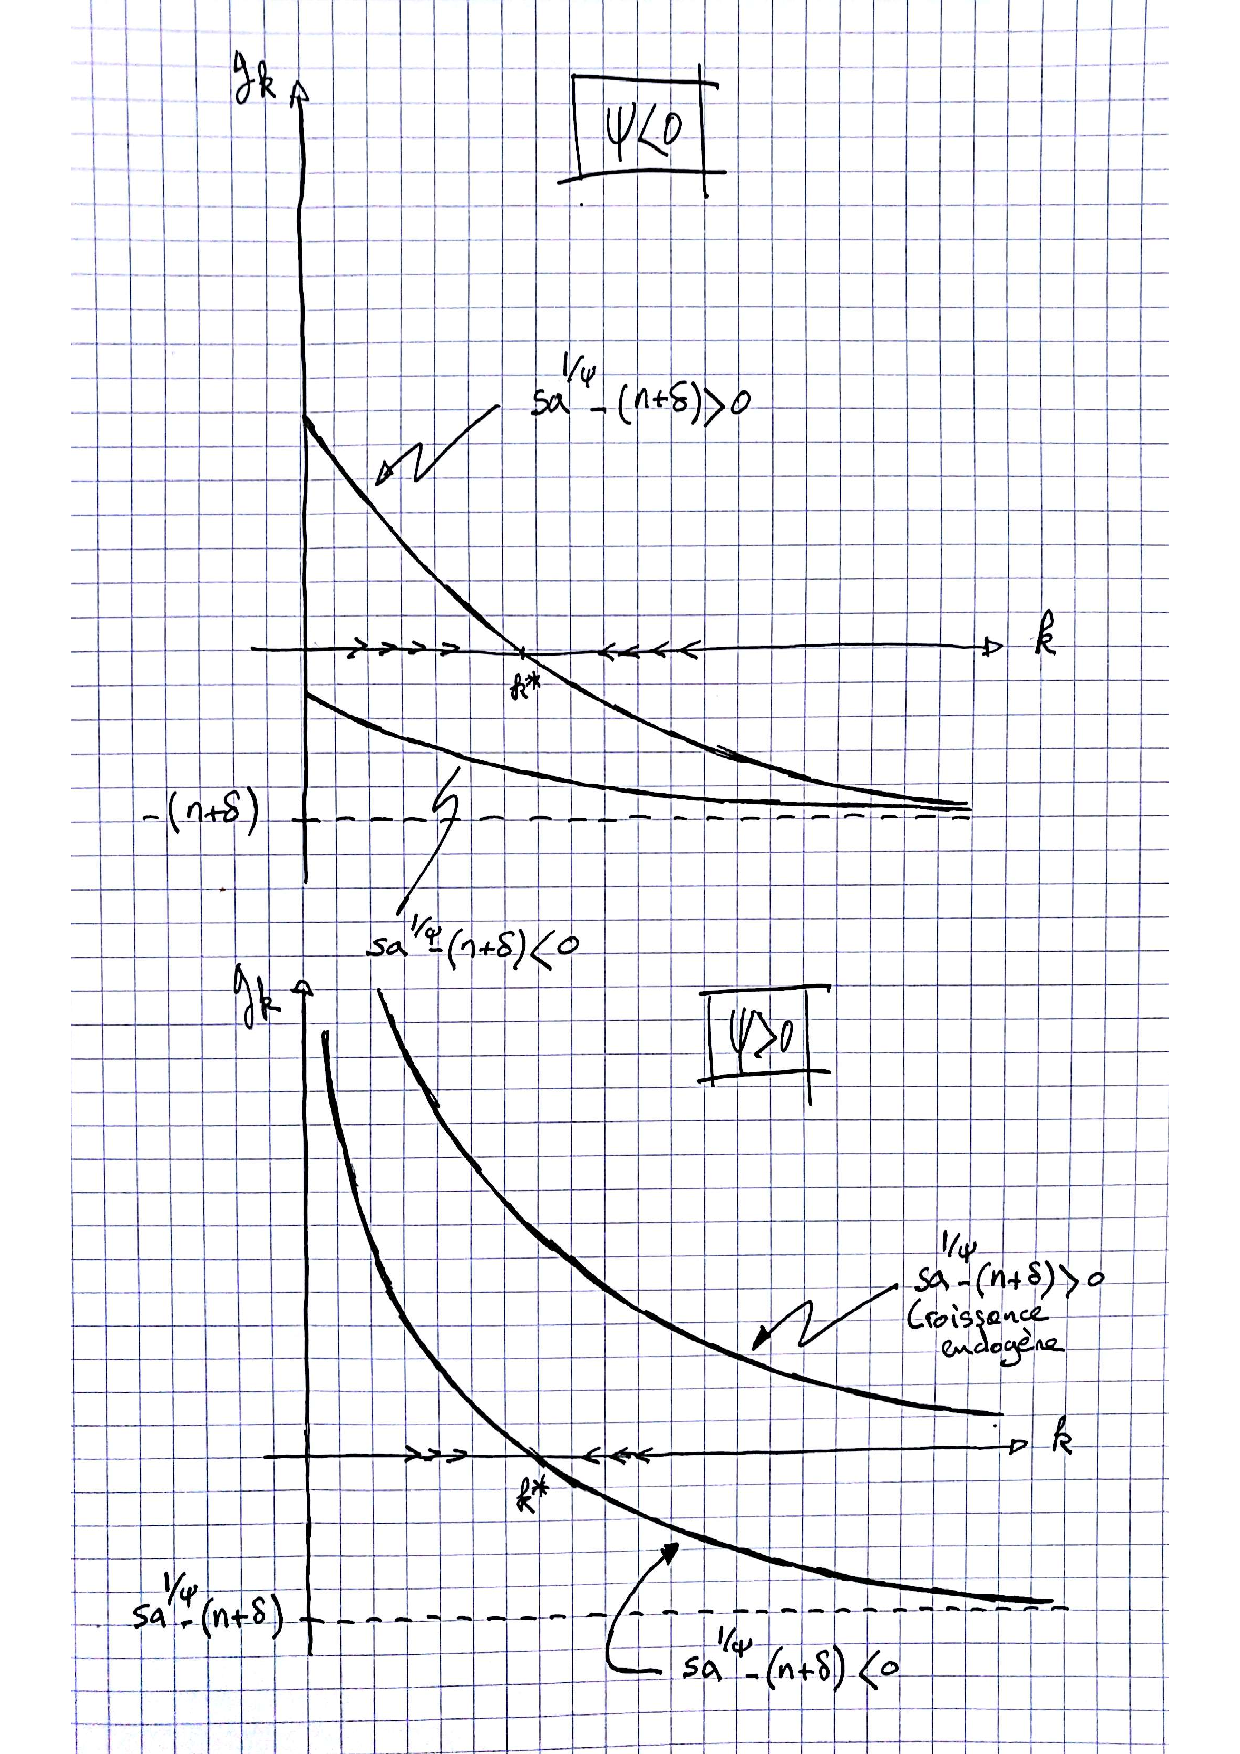
\includegraphics[scale=.7]{graphique-rattrapage-2017.pdf}


\end{document}